\def\year{2018}\relax
%File: formatting-instruction.tex
\documentclass[letterpaper]{article} %DO NOT CHANGE THIS
\usepackage{aaai18}  %Required
\usepackage{times}  %Required
\usepackage{helvet}  %Required
\usepackage{courier}  %Required
\usepackage{url}  %Required
\usepackage{graphicx}  %Required
\usepackage{fancyhdr,graphicx,amsmath,amssymb}
\usepackage[ruled,vlined]{algorithm2e}
\include{pythonlisting}
\frenchspacing  %Required
\setlength{\pdfpagewidth}{8.5in}  %Required
\setlength{\pdfpageheight}{11in}  %Required
%PDF Info Is Required:
  \pdfinfo{
/Title (2018 Formatting Instructions for Authors Using LaTeX)
/Author (AAAI Press Staff)}
\setcounter{secnumdepth}{0}  
 \begin{document}
% The file aaai.sty is the style file for AAAI Press 
% proceedings, working notes, and technical reports.
%
\title{Election Control: Attacking and Defending\\ Elections using Linear Programming}
\author{Trevor Larsen and Zach Mekus\\
Washington University in St. Louis
}
\maketitle
\begin{abstract}
For our project, we are doing an implementation of the paper Optimal Defense Against Election Control by Deleting Vote Groups by Yin et. al. The paper introduces a double oracle approach for solving the optimization problem of how to deploy defense resources to defend an election. We are implementing this double oracle algorithm, and using it on datasets from the 2016 presidential election. We create some of our own experiments, testing how the algorithms performs as a function of iteration count.
\end{abstract}

\section{Introduction}
\subsection{The Problem}

In recent centuries, the majority of governments in the world have shifted to forms of government that rely on elections. In order for democratic institutions to maintain their integrity, these elections must be both free and fair, as well as protected from outside interference. Malicious attackers may have motivation to influence the outcome of an election in a certain direction by subverting the democratic process. Examples of this include attacks on voting day in 2013 in Pakistan, where bombings killed or injured over 150 people, as well as in 2010 Sri Lanka elections where there were over 250 incidents of poll-related violence. Cyber attacks on electronic voter systems are also a threat, and while no known attacks have been  in the United States, these may prove to be targets in the future, as recent investigations have found these systems to be vulnerable. 

An attacker can attack an election with the goal of either making a certain candidate the winner, which we refer to as constructive control, or to prevent a certain candidate from winning, which we call destructive control. We are interesed in the specific example of the United States presidential election, in which we will only consider the Democratic and Republican parties. In this case, making one candidate win is equivalent to making the other candidate lose, so constructive and destructive control are equivalent. In this project, we wish to investigate how we can model an attack or defense of a presidential election in the United States, using data from the 2016 United States presidential election, specifically for Michigan and Georgia, which proved to be interesting test cases for the algorithm due to the distribution of votes.

\subsection{Related Work}

The first set of prior work we will look at is papers regarding election control. The Optimal Defense paper examines the problem of protecting elections against subversion by abstracting the process of enhancing security at voting locations, either physically or electronically. Prior work included Bartholdi et al. which looked at the problem from the point of view of computational (2015) were the first to look at election control at the level of voter groups, and grouped voters by a bundling function. In the paper of Yin et al. used a function where voting groups did not overlap, and where given voting groups were deleted by the advsersary ~\cite{article}. Erdélyi et al. added or deleted voter groups in his study, but only considered constructive control.  Yin et al. in this paper was the first to consider methods for allocating defense resources for protecting given locations in an election. Elkind and Lipmaa try to make elections more difficult to subvert by developing rules that are NP-hard to manipulate, which is different from this paper, which looks at using defensive resources to reduce likelihood of an adversary changing the out come by attacking groups.

Next we will look at papers regarding physical security problems using Stackelberg games. Prior work has looked at the problem of attackers being limited to one location, whereas in Yin et al.the attackers attack multiple locations simultaneously. Other prior work has looked at simultaneous move games or have only used heuristic approaches. Other Stackelberg games have used double oracle solutions in the past, but the unique formulation of this problem requires a unique algorithm to find an optimal solution.

\section{Model}
\subsection{Stackelberg Game Background}
In the following section, we introduce the concept of a Stackelberg game, which we will use in the model for our election control problem. A Stackelberg game consists of two players, a leader and a follower, who each decide on a strategy for the game. The leader goes first, picking a strategy, and the follower responds with a strategy. The strategies used can either be pure strategies, where players commit to a particular action, or a mixed strategy, where players choose a probability distribution over pure strategies. A Stackelberg security game is a model for an interaction between a defending security force and an adverserial attacker. In a Stackelberg security game, because the attacker picks second, they always are able to pick the action that gives them the highest probability of success due to their knowledge of the defender's strategy, and thus will always pick a pure strategy. In contrast, the defender doesn't have any such commitment from the attacker, and usually chooses a mixed strategy to minimize the attacker's probability of success, since the defender knows the attacker will exploit any weaknesses the defender leaves in his strategy. 

Let S be the set of all defender pure strategies, and A be the set of all attacker strategies. Given a defender's mixed strategy $P$ over pure strategies in $S$, $P = \{p(s) : s \in S\}$, where $p(s)$ is the probability of choosing strategy s, an attacker's action $a \in A$, and utility payoff functions for the defender $U^D(s,a)$ and attacker $U^A(s,a)$ for given pure strategy $(s,a)$ pairs we can calculate the utility of the defender and attacker:

\begin{equation}
u^D(P,a) = \sum_{s \in S}p(s)U^D(s,a)
\end{equation}
\begin{equation}
u^A(P,a) = \sum_{s \in S}p(s)U^A(s,a)
\end{equation}

let $br(P) \mapsto a$ be a function mapping a mixed strategy to the attacker's best response a. For a given mixed strategy, action pair (P,br(P)) to be a Strong Stackelberg Equilibrium it must fullfill the following criteria: 

\begin{itemize}
\item $U^D(P,a) \geq U^D(P*,br(P*))$ for any other P*.
\item The attacker's response $br(P) \in argmax_{a \in A}u^A(P,a)$
\item defender wins ties $U^D(P,br(P)) \geq U^D(P,a), \forall a \in argmax_{a \in A}u^A(P,a)$
\end{itemize}

\subsection{Model of the Election}
Yin et al. model the election as a Stackelberg security game. The election cosists of people voting at different locations. At each location, each candidate receives a certain number of votes. Attacks are modeled as a deletion of the votes at these locations. In this model for the election, the defender is the leader, and first chooses a mixed strategy over m locations to defend, with the goal of defending the outcome of the election. The attacker follows with a pure strategy, choosing which n locations to attack, trying to change the result of the election, either with the goal of having a specific candidate win (constructive control) or making a particular candidate lose (destructive control). In our case, since we are modelling the US presidential election and are only considering the Republican and Democratic party candidates, we are treating the destructive and construct control cases as the same, as they become the same problem in a 2 party-election. We model each state as being an independent election composed of the districts in each state, using data compiled by Daily Kos. For simplicty, we only consider Democratic and Republican vote tallies, and use as input to the algorithm the difference in vote tallys for each district. Each state has $D_n$ defender resources that it may allocate to defend the result of the election, while the attacker has $A_n$ attacker resources to consider to flip the result of the election in that state. 
\section{Algorithm}

In order to solve this problem, we solve a linear program which we will call Core-LP. This Core-LP takes as input the set of strategies to consider for both the attacker and the defender, as well as the vote tally difference in each district. Given these strategies and vote tallys, Core-LP computes the best defensive strategy against a following attacker, and by virtue of the dual solution, the best attacking strategy against a following defender. 

Core-LP has issues with scalability, as computational time grows exponentially with the number of strategies for both the attacker and the defender. Thus, for sufficiently large elections, this linear programming approach on its own will become intractable. In their paper, Yin et al. propose a double oracle approach to solve for optimal defense and attack strategies, using heuristics to slowly grow the number of cosidered strategies. This approach involves the use of several problem-agonstic functions which must be specified for a given problem. These algorithms are the Attack-MILP,Defense-MILP,AO-Better and DO-Better functions. We cover the implementation of the functions we have implemented so far. We present the double oracle approach in Figure \ref{fig:doubleoracle}. In each iteration, the approach adds new best response pure stratgies for both the attacker and the defender to the list of considered strategies by executing AO-Better and DO-Better. If either AO-Better or DO-Better is unable to find an improved strategy, they pass off work to Attack-MILP or Defense-MILP respectively, which will return a pure strategy for the attackers and defenders to consider in the Core-LP. Once the approach is unable to find new strategies that improve upon the current set of strategies and actions, the approach terminates, returning the mixed strategy calculated by Core-LP for the defender. 

\begin{figure*}[!h]
  \centering
  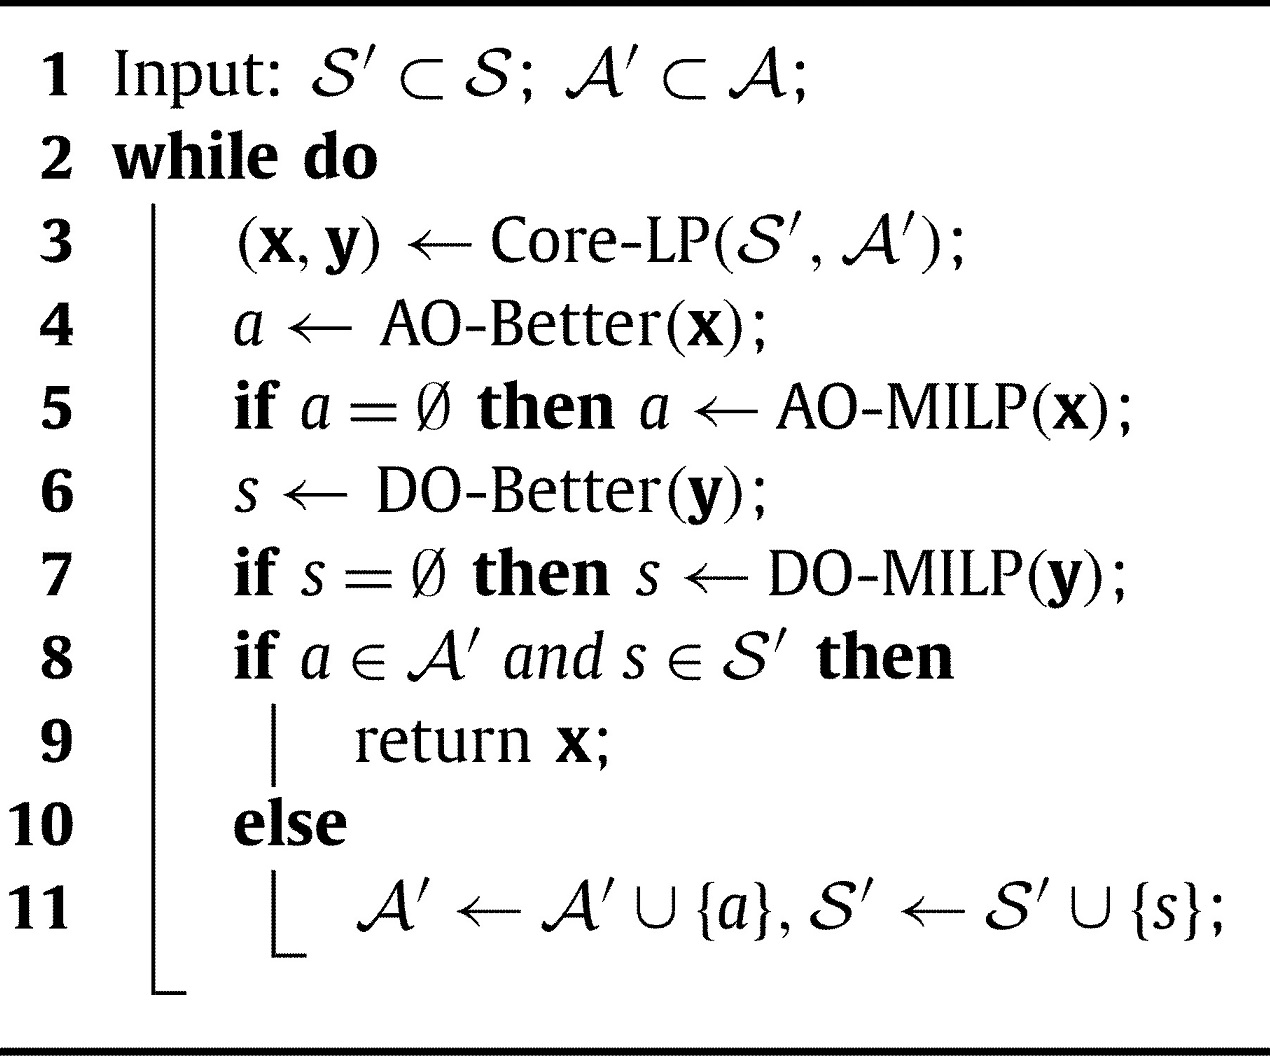
\includegraphics[height=10em]{doubleoracle.jpg}
  \caption{The double oracle algorithm proposed by Yin et al.}
  \label{fig:doubleoracle}
\end{figure*}

\subsection{Attack-MILP}
In this section we describe our modified version of the Attack-MILP Linear Program that we developed for the 2-candidate scenario. In this version, we explicitly write out the linear version of the optimization problem in the original paper and removed variables that aren't relevant in a 2-candidate scenario. Attack-MILP takes as input a mixed defense strategy generated by Core-LP. The Linear Program is given below.
Let $x_j$ be the probability of the jth defensive strategy being played. Let $a_i$ be 1 if attack action i is taken, and 0 otherwise. Let $t_i$ be the difference in vote count for district i. $z_j$ is 1 if the attacker will win against pure defense strategy j. $v_{ij}$ is a linearization variable that is 1 if district i is attacked with defense j, and will win the attack, and is calculated as $v_{ij} = a_iz_j$. $S_{ij}$ denotes whether district i is defended in strategy j. k is the maximum number of attacks the attacker may execute. 

Attack-MILP seeks to minimize the objective function:
\begin{equation}
min_{a_i,z_j,v_{ij} \in \{0,1\}}\sum_{j}(1-z_{j})x_j \\
\end{equation}
subject to the following constraints:
\begin{equation}
\sum_{i}a_{i} \leq k
\end{equation}
\begin{equation}
\sum_{i}(z_jt_i-(1-S_{ij})v_{ij}t_i) \geq 0 \forall j
\end{equation}
\begin{equation}
v_{ij} \leq z_j \forall i,j
\end{equation}
\begin{equation}
v_{ij} \leq a_i \forall i,j
\end{equation}
\begin{equation}
v_{ij} \geq z_j+a_i-1 \forall i,j
\end{equation}


\subsection{Defense-MILP}

Let $y_j$ be the probability of the jth attack strategy being played. Let $s_i$ be 1 if defensize action i is taken, and 0 otherwise. Let $t_i$ be the difference in vote count for district i. $z_j$ is 1 if the defender will win against pure attack strategy j. $v_{ij}$ is a linearization variable that is 1 if district i is defended with attack j, and will win the defense, and is calculated as $v_{ij} = s_iz_j$. $A_{ij}$ denotes whether district i is attacked in strategy j. $l$ is the maximum number of attacks the attacker may execute. 
Defense-MILP seeks to maximize the objective function:
\begin{equation}
max_{s_i,z_j,v_{ij} \in \{0,1\}}\sum_{j}z_{j}y_j \\
\end{equation}
subject to the following constraints:
\begin{equation}
\sum_{i}s_{i} \leq l
\end{equation}
\begin{equation}
\sum_{i}(z_jt_i(1-A_{ij}) + v_{ij}t_iA_{ij} + z_j \leq 0 \forall j
\end{equation}
\begin{equation}
v_{ij} \leq z_j \forall i,j
\end{equation}
\begin{equation}
v_{ij} \leq s_i \forall i,j
\end{equation}
\begin{equation}
v_{ij} \geq z_j+s_i-1 \forall i,j
\end{equation}

\subsection{AO-Better}
In this section we describe the modified AO-Better heurisitic for generating attack strategies. The goal of AO-Better is to provide a heuristic that can be calculated quickly to generate new attacks that are better than attacks that have already been added to the set of Attack $A'$. In AO-Better, the set of defender strategies S' is sorted in decreasing order of $X_s$, and we call this sorted set $\bar{S}$. The algorithm then looks for adjacent strategies in $\bar{S}$, called $S''$ such that if an attack exists that would flip the electon to the attacker's favor for any strategy $s \in S''$, and returns the attack the would flip the electon in all cases for that subset of strategies $S''$. In the double oracle algorithm, if an attack is unable to found by AO-Better, AO-MILP will find the optimal attack. Our modified algorithm for the 2-candidate case is shown below.

\begin{algorithm}
\SetAlgoLined
\KwResult{heuristic attack strategy a }
 Input: S',x,p\;
$\bar{S} =  \langle s^{\rho}, \rho \in 1, 2, 3, ...\rangle \leftarrow s \in S'$ by decreasing $x_s$;\
\For{$\rho$ in 1..$|\bar{S}|$}{
 $p' \leftarrow x_{s^\rho}$\;
 $S'' \leftarrow \{s^{\rho}\}$\;
$\rho' \leftarrow \rho' + 1$\;
\While{$p' \leq 1 - p$ and $\rho \leq |\bar{S}|$}{
$p' \leftarrow p' + x_{s^\rho}$\;
$S'' \leftarrow S'' \cup \{s^{\rho'}\}$\;
$\rho' \leftarrow \rho' + 1$\;
  \If{$p' > p$}{
   	$t \backslash k \leftarrow$ delete k elements in t with smallest $t_i$ and $s_i = 0$\;
	\If{sum($t\backslash k) \geq 0$}{
		\Return attack corresponding to deleted elements
	}
   }{
  }
 }
}
\Return $\emptyset$
 \caption{AO-Better}
\end{algorithm}


\subsection{DO-Better}
In this section we describe the modified DO-Better heuristic for generating defense strategies. The goal of DO-Better is to provide a heuristic that can be used to quickly calculate new defenses that can defend successfully against a subset of attacks. DO-BETTER works as follows. First, the powerset of all attacks that have a probability of occuring are generated. For each subset in this powerset with $\sum_{a \in A''} y_a > p$ we look for a defense strategy s that can block every attack in $A''$, this will guarantee that the candidate the defender is defending will win with probability at least p. If a defense is unable to be found by the heuristic algorithm, Defense-MILP is ued to find the optimal defense strategy. Our simplified version of the algorithm for two candidates is given below. 

\begin{algorithm}
\SetAlgoLined
\KwResult{heuristic defense strategy s }
$s =  \langle s_{i} = 0: \forall i \in {1,...,n}\rangle$\; 
PS = powerset(A')\;
\For{$A''$ in PS with $\sum_{a \in A''} y_a > p $}{
res = 0\;
t' $\leftarrow \langle t_i : i$ with $a_i =0, \forall a \in A''$  or $s_i = 1 \rangle$;\ 
\While{sum(t') $\geq 0$ and $res < m$}{
$t'' \leftarrow t \backslash t'$\;
$ i^* \leftarrow argmin_i\{t''\}$\;
$t' \leftarrow t' \cup \{t_i^*\}$\;
$s_i^{*} \leftarrow 1$\;
$res \leftarrow res + 1$\;
}
  \If{$sum(t') <  0$}{
	\Return s
   }
 }
\Return $\emptyset$
 \caption{DO-Better}
\end{algorithm}



\section{Results/Evaluation}

\begin{figure}
    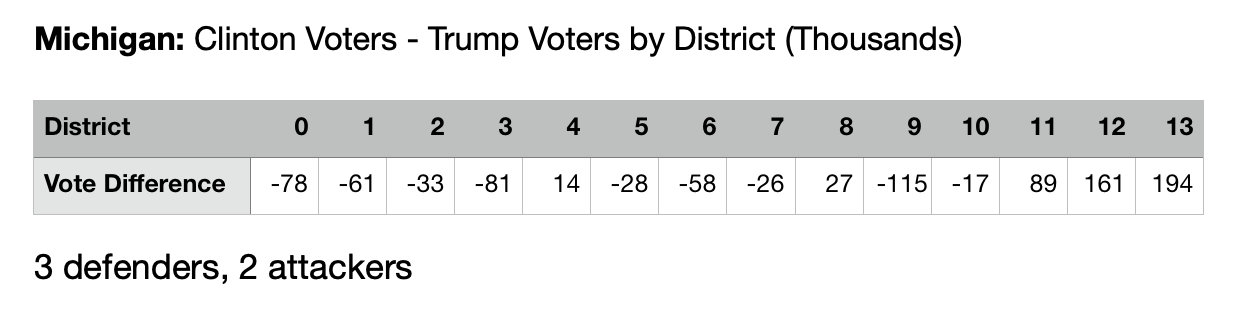
\includegraphics[width=\linewidth]{michigan_votes}
    \label{michigan_votes}
    \caption{difference in voter totals for Michigan}
\end{figure}

\begin{figure}
    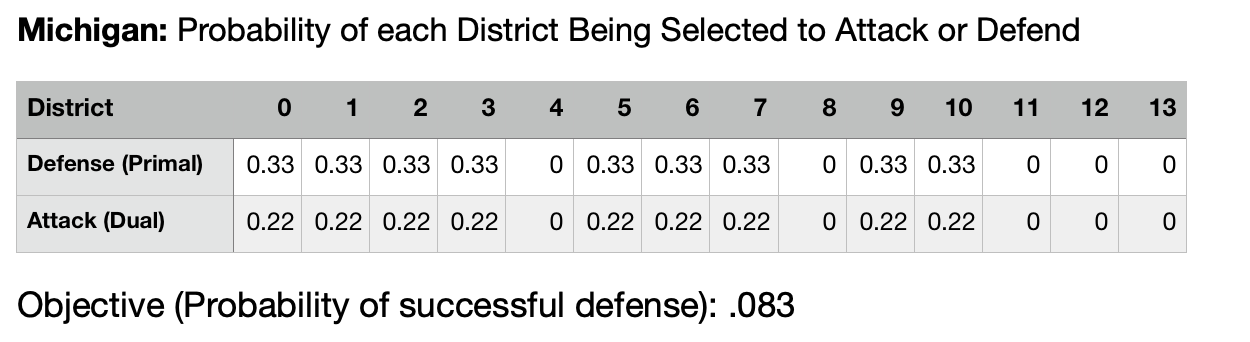
\includegraphics[width=\linewidth]{michigan_probs}
    \label{michigan_probs}
   \caption{Michigan district attack and defense probabilities}
\end{figure}

\begin{figure}
    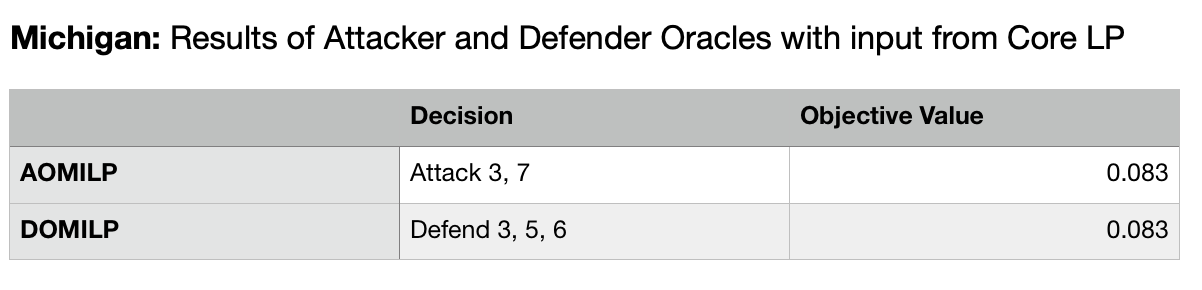
\includegraphics[width=\linewidth]{michigan_oracles}
    \label{michigan_oracles}
    \caption{AOMILP and DOMILP results}
\end{figure}

\begin{figure}
    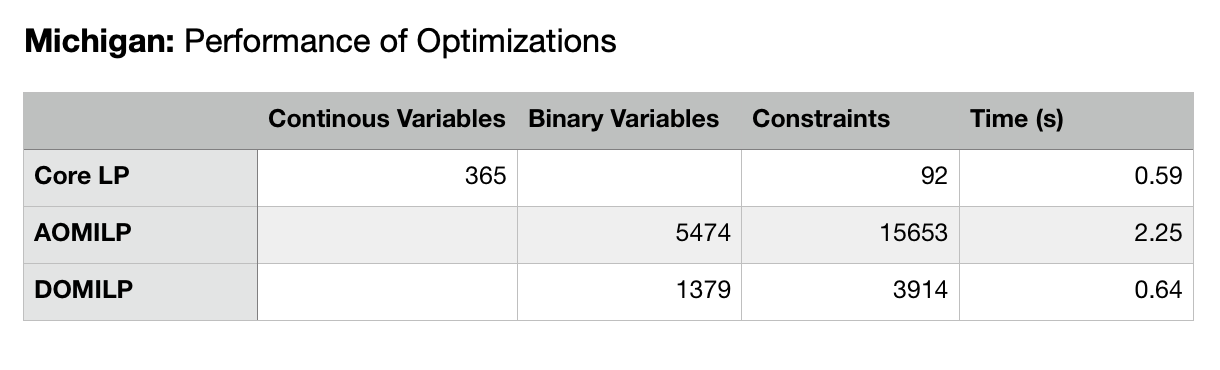
\includegraphics[width=\linewidth]{michigan_perfs}
    \label{michigan_perfs}
    \caption{Performance of Core LP and AOMILP/DOMILP}
\end{figure}

\begin{figure}
    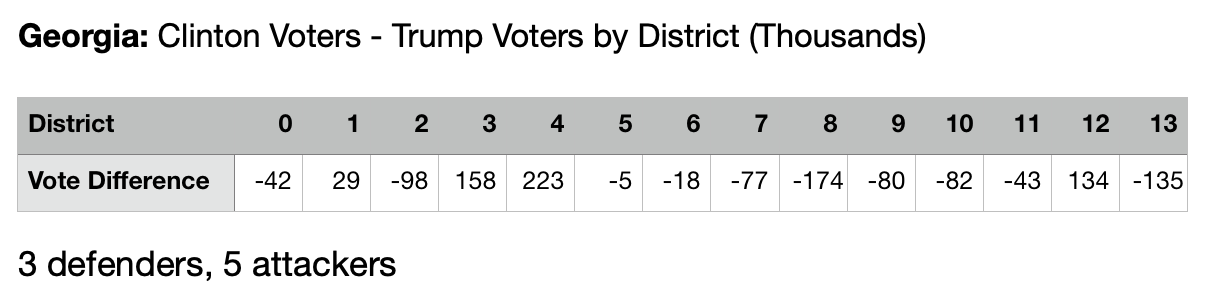
\includegraphics[width=\linewidth]{georgia_votes}
    \label{georgia_votes}
   \caption{difference in voter totals for Michigan}
\end{figure}

\begin{figure}
    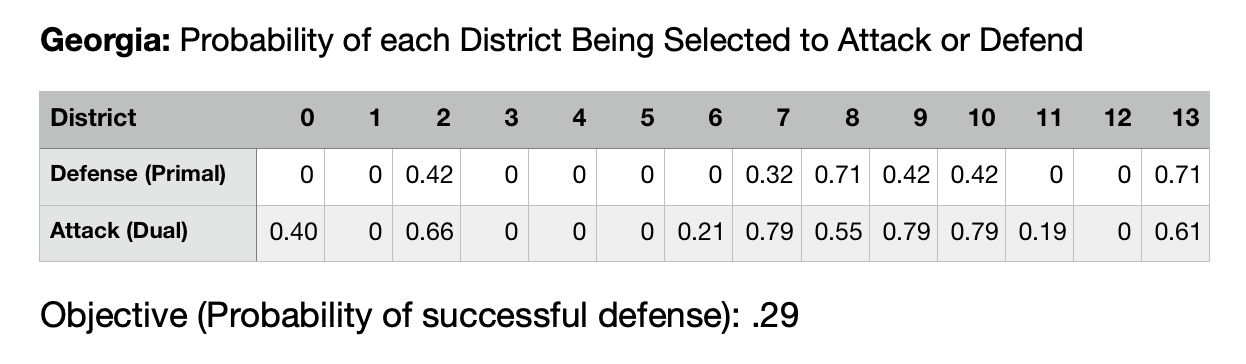
\includegraphics[width=\linewidth]{georgia_probs}
    \label{georgia_probs}
   \caption{Michigan district attack and defense probabilities}
\end{figure}

\begin{figure}
    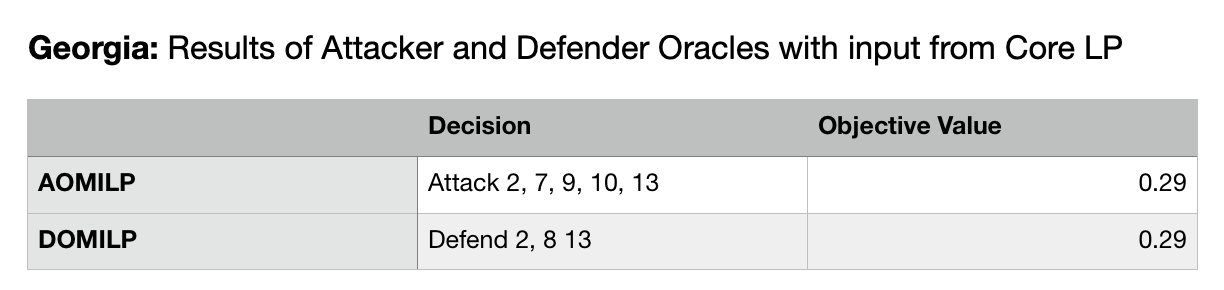
\includegraphics[width=\linewidth]{georgia_oracles}
    \label{georgia_oracles}
\caption{AOMILP and DOMILP results}
\end{figure}

\begin{figure}
    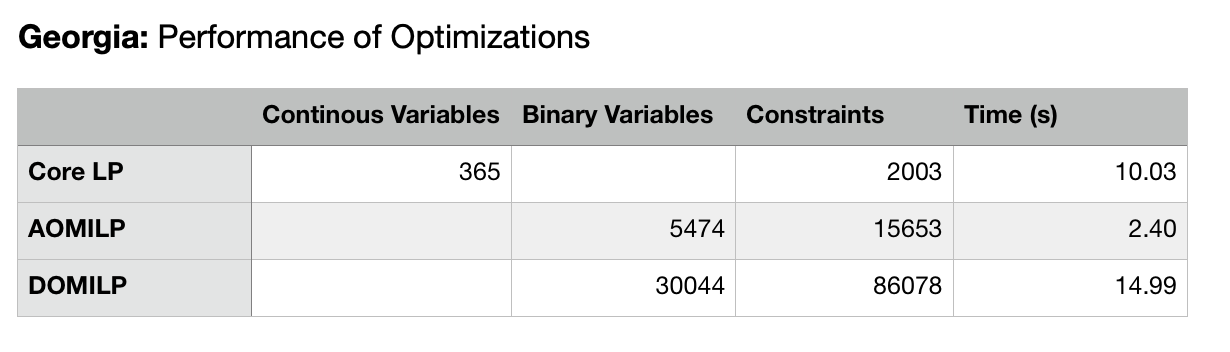
\includegraphics[width=\linewidth]{georgia_perfs}
    \caption{Performance of Core LP and AOMILP/DOMILP}
    \label{georgia_perfs}
\end{figure}


\begin{figure}
    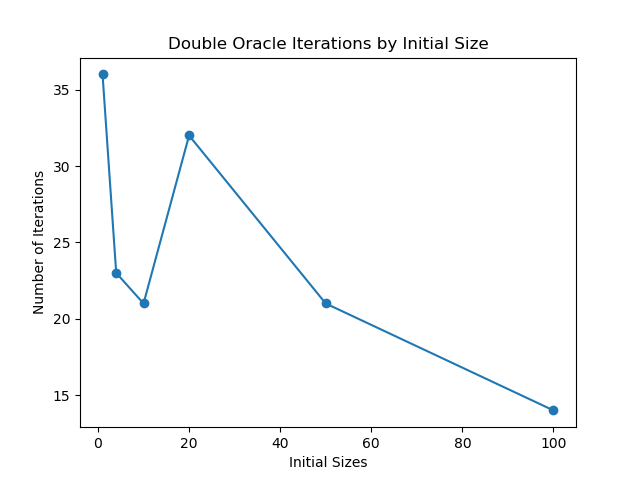
\includegraphics[width=\linewidth]{oracle_its}
    \label{oracle_its}
    \caption{number of iterations for double oracle approach as function of starting input size for A', S'}
\end{figure}

\begin{figure}
    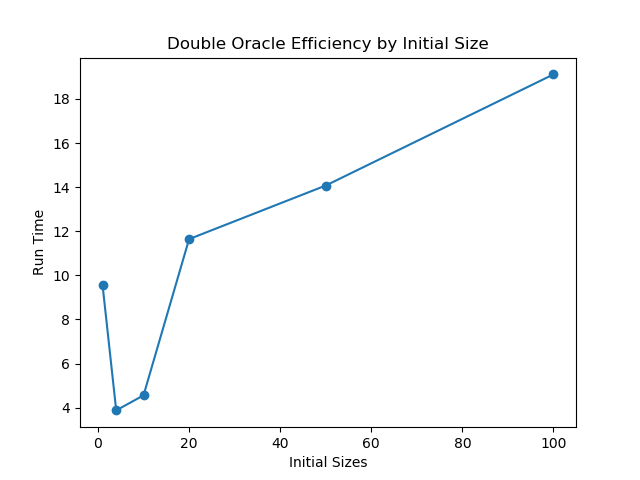
\includegraphics[width=\linewidth]{oracle_times}
    \label{oracle_times}
    \caption{Runtime for double oracle approach as function of starting input size for A', S'}
\end{figure}




\subsection{Overview}

The results section has the following goals: To show that what has been implemented is correct, to get an initial evaluation of our states data, and to gauge the limitations of Core LP in terms of run time. We evaluate on 2016 US presidential election data using the difference in votes between Hillary Clinton and Donald Trump in each congressional district of the states Michigan and Georgia. The optimal randomized defensive strategy is solved using Core LP and the dual solution of Core LP is the optimal randomized attacking strategy for the scenario where the attacker moves first and the defender plays a pure strategy. AOMILP and DOMILP work by taking as input a set of strategies and returning the optimal attacking and defending strategy respectively. In the double oracle approach a set of initial strategies and attacks are chosen from the set of all possible strategies and attacks. heuristic strategies add to this set very quickly, and if they fail, AOMILP and DOMILP add optimal attacks and defense strategies, albeit slower. The probability vectors over the districts are calculated by finding the expectation that each district will be defended or attacked based on the randomized strategy.

\subsection{Michigan}

In 2016 the presidential election results went narrowly to Donald Trump. If any district that favored Trump is deleted, the results would have changed. Here we use three defenders and two attackers, but the results would have been similar no matter what. Since every district is equally valuable, the defenders and attackers pretect them equally. Table \ref{michigan_probs} shows the equal distribution among districts the defender won, in both the attacking and defending solutions (defending sums to 3, attacking sums to 2). This is also seen in the response in table \ref{michigan_oracles} by the attacker and defender, which arbitrarily choose districts among those the defender won. 

\begin{figure}
    \includegraphics[width=\linewidth]{georgia_districts}
    \label{georgia_districts}
   \caption{difference in voter totals for Michigan}
\end{figure}

\begin{figure}
    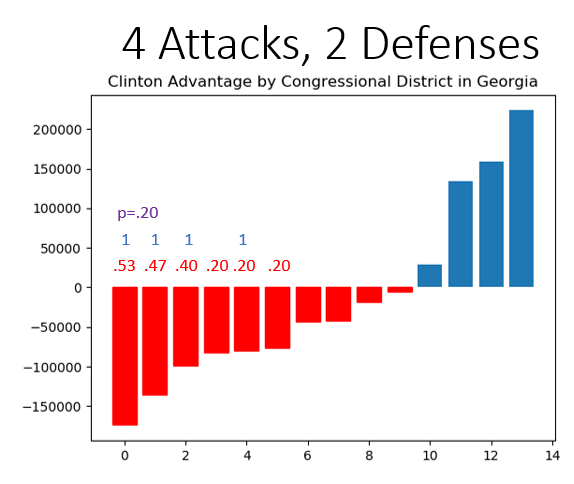
\includegraphics[width=\linewidth]{4and2}
    \label{4and2}
    \caption{attack and defense strategy results for 4 attacks and 2 defense in Georgia.}
\end{figure}

\subsection{Georgia}

While Georgia was competitive, it wasn't so close that any flipped district would change the outcome. The distribution of voter advantages by district can be seen in Figure \ref{georgia_districts}. To induce a more interesting result, 3 defenders and 5 attackers were introduced and this resulted in a 29\% chance of defending successfully. As seen in table \ref{georgia_probs} the larger defender-won districts got more defense and attack. Because the attackers had more options, they could sometimes attack districts never defended. Table \ref{georgia_oracles} shows that each of the oracles corresponds to choosing the most attacked/defended districts, but not neccessarily the ones with the most votes to destroy. 



\begin{figure}
    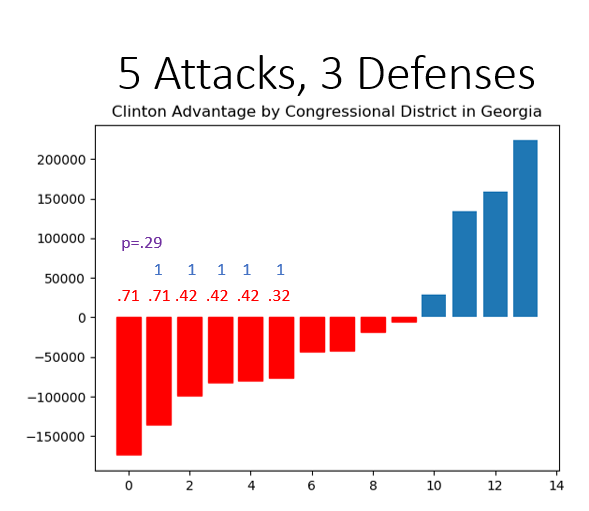
\includegraphics[width=\linewidth]{5and3}
    \label{5and3}
 \caption{attack and defense strategy results for 5 attacks and 3 defense in Georgia.}
\end{figure}

\begin{figure}
    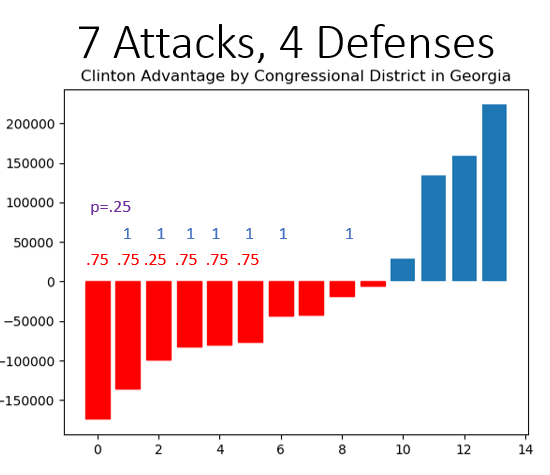
\includegraphics[width=\linewidth]{7and4}
    \label{7and4}
 \caption{attack and defense strategy results for 7 attacks and 4 defense in Georgia.}
\end{figure}


\subsection{Double Oracle Efficiency and Iterations as a function of initial size}

The Double Oracle algorithm tasks as input a starting of attack and defense strategies A' and S'. The paper did not specify how to decide on these values. We decided to see how changing the number of starting attack and defense strategies changes the number of iterations to convergence as well as the efficiency measured by runtime. The results of these experiments can be seen in Figure \ref{oracle_its} and Figure \ref{oracle_times}. Number of initial attacks and defenses was set to 1, 4, 10, 20, 50 and 100. The number of iterations taken to find the optimal solution reached a minimum of iterations of 15 when initialize size was set to 100, and seemed to follow a negative linear trend.. There was also another local minimum at 10 iterations.  \\
Runtime reached a minimum at 4 iterations. and increased as a function of initial size. Generally speaking, the optimal solution for balancing runtimes and number of iterations seemed to be to start the approach with four attack strategies and four defense strategies. The double oracle approach, when optimized with good initial sizes ran an order of magnitude faster than using Core LP on its own. This can be seen in Figure \ref{timingdifferences}

\begin{figure}
    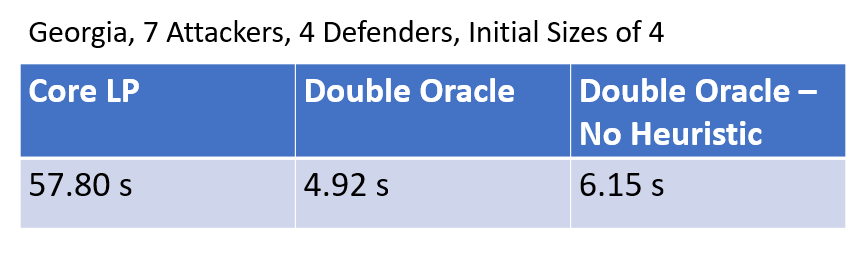
\includegraphics[width=\linewidth]{timingdifferences}
    \label{timingdifferences}
    \caption{Runtime of Core LP vs Double Oracle approach for Georgia, 7 attackers, 4 defenders}
\end{figure}

\subsection{Results Conclusion}

The two oracles AOMILP and DOMILP appear to have performed correctly, especially by getting the same optimal value as Core LP. As expected, with more defender and attacker strategies, the optimizations of Georgia took longer to compute. This certainly seems to be a limitation on the future of using Core LP on larger states or using lower level districts like counties.


\section{Related Work}

We experiment on the same data as Yin et al. with 2016 Michigan presidential data. With the same settings, three defense and two attack resources, we both get the same result of .29 success rate. This is promising as it serves as further confirmation that we have implemented Core LP corectly. In the Results section, we expand on the choices made by the defensive and attacking agents in Michigan and Georgia to further understand the process. In the future, we hope to expand on solving this problem for all states. 

\section{Conclusion, Limitations, and Future Work}
In summary, the improvd runtime of the double oracle approach is dependent on the initial attacker and defender strategy setup. One limitation of the approach we have taken is that runtime can still be prohibitive for states with many districts. Additionally districts are a poor representation of voting units since a district has many counties within it, and counties have many voting centers within them. Analyzing group voting at the level of voting centers is far more realistic, though computationally much more porhibitive. Additionally, it is difficult to find voting data at the level of individual voting centers. Counties are also too numerous to be computationally tractable for a project with our computational resources. Future work for this project could include expanding this approach to a nationwide election, modelling attacker and defender resources by states, and implementing a heuristic at the national election level for deciding on swing states to attack.
{
\bibliographystyle{aaai}
\bibliography{election}
}



\end{document}
